\documentclass[a4paper,11pt]{kth-mag}
\usepackage[T1]{fontenc}
\usepackage{textcomp}
\usepackage{lmodern}
% \usepackage[latin1]{inputenc}
\usepackage[utf8]{inputenc}
\usepackage{url}
\usepackage[german,english,swedish]{babel}
\usepackage{modifications}
\usepackage{float}
\usepackage{listings}
\usepackage{msc}

\usepackage{graphicx}
\usepackage{geometry}
\usepackage{pdflscape}
\usepackage{cleveref}
\usepackage{csquotes}
\usepackage{subcaption}

\usepackage[printonlyused,withpage]{acronym}
\usepackage[detect-weight=true, binary-units=true]{siunitx}
\usepackage[section]{placeins}


% \includepdf{cover.pdf}

\title{Knitting Thesis}

% \subtitle{Duis autem vel eum iruire dolor in hendrerit in
%           vulputate velit esse molestie consequat, vel illum
%           dolore eu feugiat null}
% \foreigntitle{Lorem ipsum dolor sit amet, sed diam nonummy nibh eui
%               mod tincidunt ut laoreet dol}
\author{Bianca Ploch}
\date{August 2016}
\blurb{Bachelor Thesis at HTW\\Supervisor: \\Examiner: }

\begin{document}
\frontmatter
\pagestyle{empty}
\removepagenumbers
\maketitle
\selectlanguage{english}
\begin{abstract}

\end{abstract}
\clearpage

\title{Sachen Thesis}
\author{Bianca Ploch}
\date{August 2016}
\blurb{Bachelor Thesis at HTW\\Supervisor: \\Examiner: }
\maketitle

\begin{foreignabstract}{german}

\end{foreignabstract}
\clearpage

\tableofcontents*
\mainmatter


\pagestyle{newchap}
\chapter{Introduction}
\textit{This section describes the problem and research question(s) to be looked at in
this thesis.}

Nowadays we find ourselves in a very different world than even 20 years ago.
Following the rise of the mobile phone we got the smartphone, the handy pocket
computer for young and old. With technological advance came better processing
power, more storage for all the important pictures and videos in life, and the
big display to view everything in nearly lifelike colours. Together with it came
 the advent of the mobile application, more commonly referred to as an app. The
 many apps available are helpful tools to manage our daily lives and needs.
 Google’s distribution service for Android apps, the Google Play Store,
 surpassed the 1 million app mark in 2014.

But despite the many apps available, one is hard pressed to find apps concerned
with knitting, and even fewer ones that present a clear user interface or adhere
to modern design guidelines for apps. This thesis analyzed knitting related
Android apps on the Google Play Store. Most of the apps I found there do not
support the inputting or displaying of a knitting pattern chart.

The difficulty with displaying such a chart on a mobile device derives from the
size of the device and its screen, which is a far smaller medium than a sheet of
paper, on which pattern charts are normally printed. The charts are therefore too
big to be viewed easily inside an app. The goal for this thesis is to research
how a knitting pattern chart can be input and displayed on mobile Android
devices, including both phones and tablets.

\chapter{Background}
\textit{This section will give an overview of the information relevant to this
thesis’ topic.}

\section{Definition of Knitting Pattern and Knitting Pattern Chart}
A knitting pattern specifies a set of instructions outlining the steps necessary
to create a knitted textile or fabric. For knitting a fabric the knitter uses
two or more knitting needles and a long, continuous strand of yarn which he uses
to form intersecting loops with, which in turn creates a textile or fabric.
'Knitting is a conversion system in which yarn loops are interwoven to form a
fabric' ~\cite[p17]{raz1993}. The type of loops the knitter uses as well as the kind
of yarn determine the attributes of the knitted piece: elasticity, form and
texture. A knitted fabric can be stretched in both horizontal and vertical
directions, as well as the directions in-between. This makes it stand apart
from woven fabric, which are created by layering two threads in an interlaced
manner; the resulting fabric is very limited in its ability to stretch and be
formed, excluding, of course, the usage of stretching threads.

Knitting patterns can come in form of written instructions, usually with
abbreviations used for the stitch terms. e.g. k2tog for the 'knit two together'
stitch, or in form of pattern chart which consists of a grid and symbols. Both,
written patterns and pattern charts, are generally split up into rows, where
each row has a definite number of stitches. Each cell in such a grid signifies a
stitch in the pattern and the symbol displayed in a cell corresponds with the
stitch that needs to be made in that place in the pattern. In what order the
rows have to be knitted depends on the chart type; some charts display only the
uneven numbered rows, which belong to the right side (RS) of the knitted fabric,
and expect the knitter to knit the return row on the wrong side (WS) inverse to
the RS, i.e. knits would be knitted as purls and purls as knits. Other charts
show all rows, the uneven numbered for the RS and the even numbered ones for the
 WS.

So far there doesn't exist an international standard for the symbols used in
knitting charts or the abbreviations in written instructions. Symbols used by
the industry usually vary depending on the region ~\cite[p57]{raz1993}. and it is the
norm that a knitting pattern includes a glossary for the symbols and
abbreviations used in the pattern. Singular exception to this is Japan, where
there exists a Japanese Industrial Standard on knitting symbols used in the
industry and for the hobby hand knitters: JIS L 0201-1995~\cite{jkca1995}. This
leads to the fact that Japanese knitting pattern charts are published without an
index of the symbols used.

Other regional industry standards that Raz mentions in his book are the German
Standard and the needle notation system, 'the most explicit and accurate of all
 notation systems' ~\cite[p58]{raz1993}., which is solely used for industrial knitting
 and shows the positions of the needles of the knitting machine for each stitch.

\section{Comparison of existing solutions}

\subsection{Android apps}
When searching for the term ‘knitting’ in the Google Play Store, Android’s
official source for Google-approved applications, quite a few results will pop
up. Next to a surprising amount of games about knitting, there are apps for
knitting counters, knitting patterns and knitting instructions for those who
wish to begin knitting. In the following sections I will look into the top five
apps for creating and managing knitting projects with row counters and pattern
display, as well as knitting chart creation.

\subsubsection{knit tink | Row Counter by Jennifer K. Warren}
Out of all most popular knitting apps, knit tink features the most modern and
clean design. The app can be used for free or bought as an ad-free pro version.
Features include the creation, editing, viewing, and deletion of projects, the
setup of one row, and one repeat counter per project, as well as the unlinking
of the row counter from the repeat counter. The free version of the app
restricts the number of projects to three. The developer announced an on-screen
display of a knitting chart in PDF format as an upcoming feature.


\begin{figure}[H]
\centering
\begin{minipage}{.5\textwidth}
  \centering
  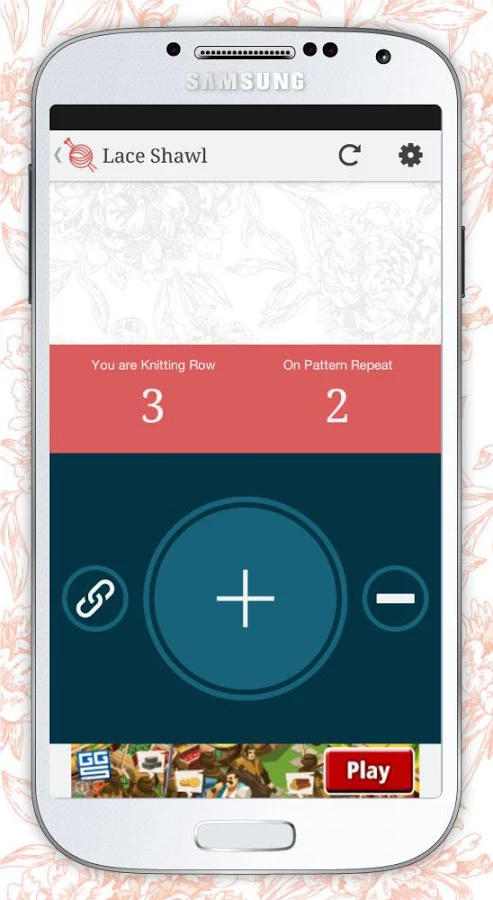
\includegraphics[width=2in]{images/image10.png}
  \caption{Row Counter of knit tink}
  \label{fig_knittink1}
\end{minipage}%
\begin{minipage}{.5\textwidth}
  \centering
  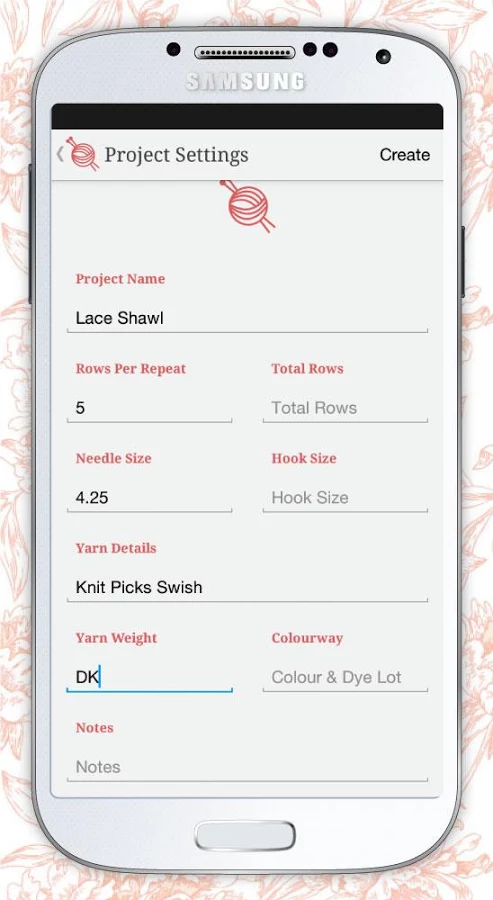
\includegraphics[width=2in]{images/image11.png}
  \caption{Project set up of knit tink}
  \label{fig_knittink2}
\end{minipage}
\end{figure}

\subsubsection{Knitting Counter by mkacki}
Knitting Counter offers the same features a the knit tink app, the only
differences being the layout of the user interface and the option to keep the
phone from going into sleep mode, i.e., turning the phone screen off.


\begin{figure}[H]
\centering
\begin{minipage}{.5\textwidth}
  \centering
  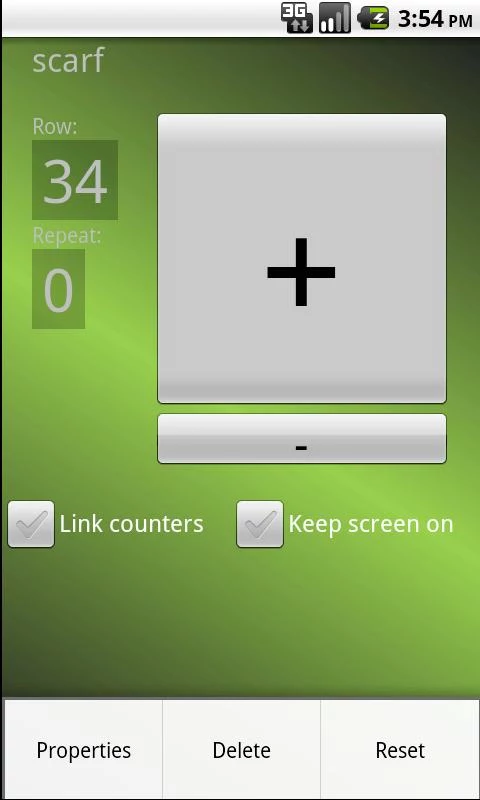
\includegraphics[width=2in]{images/image12.png}
  \caption{Counter of Knitting Counter    }
  \label{fig_knittingcounter1}
\end{minipage}%
\begin{minipage}{.5\textwidth}
  \centering
  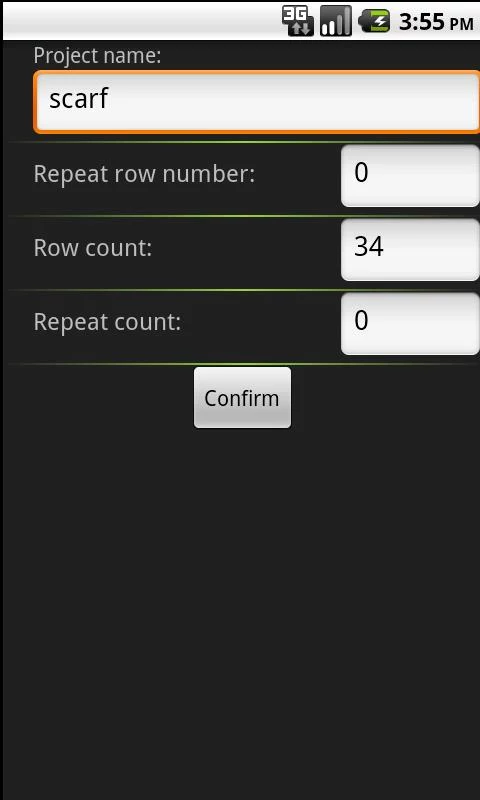
\includegraphics[width=2in]{images/image06.png}
  \caption{Counter set up screen of Knitting Counter}
  \label{fig_knittingcounter2}
\end{minipage}
\end{figure}

\subsubsection{Knitting and Crochet Buddy by Colorwork Apps}
The Knitting and Crochet Buddy contains a plethora of features related to
knitting and crocheting. As is the standard with the previous apps, it offers
the possibility to manage different knitting and crocheting projects, with each
a row and a repeat counter per project. Users can also enter written
instructions or add a picture of the pattern chart to be displayed on the
counter screen.

Additional features include, but are not limited to: yarn and crochet charts,
an abbreviation chart, size charts for knitting needles and crocheting hooks,
a project timer, a ruler function, and a flashlight.

\begin{figure}[H]
\centering
\begin{minipage}{.5\textwidth}
  \centering
  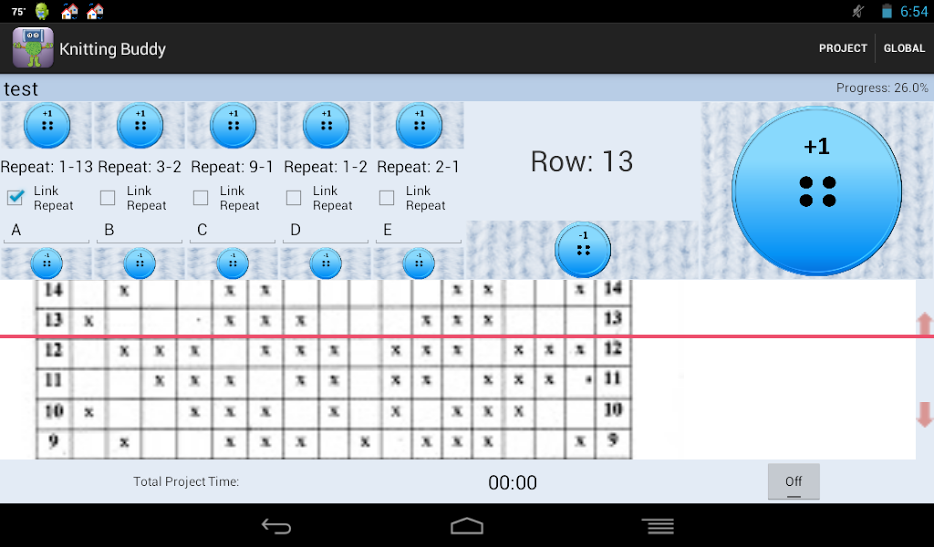
\includegraphics[width=2in]{images/image04.png}
  \caption{Counter of Knitting Buddy with written instructions}
  \label{fig_knittingbuddy1}
\end{minipage}%
\begin{minipage}{.5\textwidth}
  \centering
  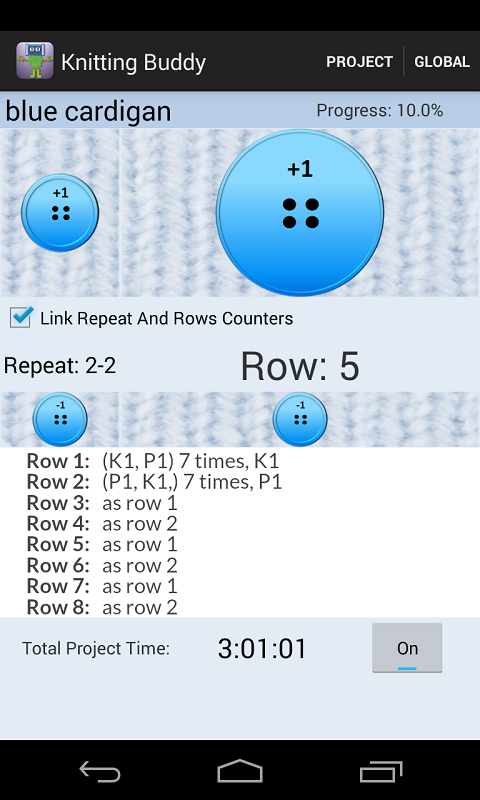
\includegraphics[width=2in]{images/image05.png}
  \caption{Counter of Knitting Buddy with chart picture}
  \label{fig_knittingbuddy}
\end{minipage}
\end{figure}


\subsubsection{BeeCount knitting Counter by knirirr}
BeeCount differs from the standard of one row counter per project in that it
allows multiple counters. Those counters can be for parts of the knit piece that
 belong to the same project, as is the case for a knitted sweater, for example.
These counters within a project can be linked together, so that increases or
decreases in one counter affect the row number of another counter (figure 8).
Furthermore, alerts can be set on counters to be triggered once the counter
reaches a set number.


\begin{figure}[H]
\centering
\begin{minipage}{.5\textwidth}
  \centering
  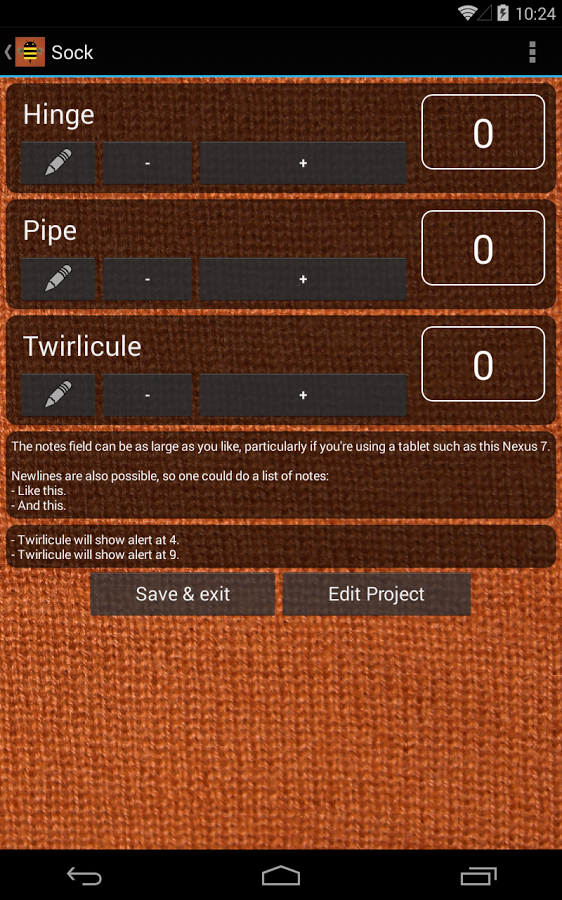
\includegraphics[width=2in]{images/image01.png}
  \caption{Counters of BeeCount}
  \label{fig_beecount1}
\end{minipage}%
\begin{minipage}{.5\textwidth}
  \centering
  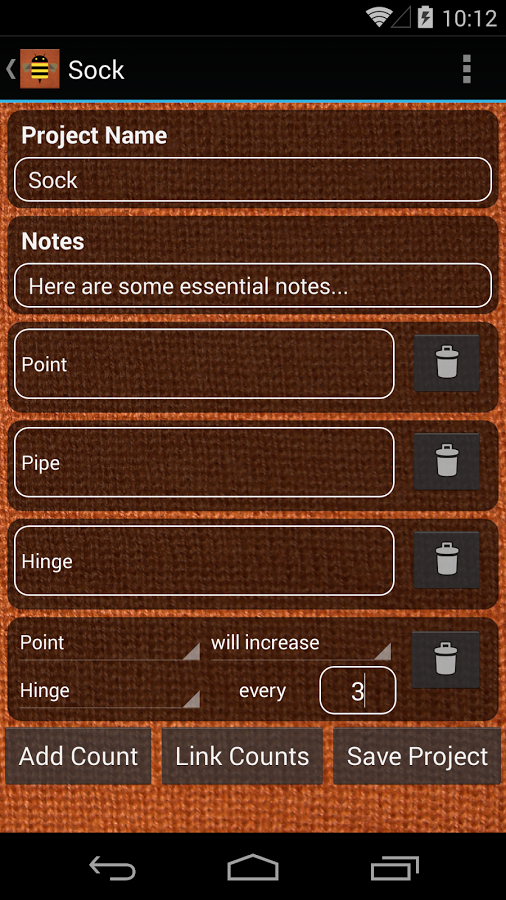
\includegraphics[width=2in]{images/image07.png}
  \caption{Counters set up of BeeCount}
  \label{fig_beecount2}
\end{minipage}
\end{figure}


\subsubsection{Knitting Chart Maker by Awesome Applications}
When it comes to pattern charts, none of the aforementioned apps offers a
solution besides the possibility to include a picture of a pattern. Therefore, I
looked at Knitting Chart Maker, an app that focuses solely on the creation and
editing of charts.

The app has over 30 stitch symbols that the user can use to create a pattern
hart. The symbols are defined by the app and are not taken from a standard. The
user can’t devise their own stitch symbols. Symbols can be used by selecting
the symbol in the left-hand menu and then transferred onto the grid by tapping
on a cell. Alternatively, the user can select the paintbrush button on the
top-left menu and use their finger to paint the symbols onto every cell touched
in a swiping motion, not unlike drawing with a pencil. The whole grid is
zoomable up to a certain zoom level.

While in-app, the user can purchase the pro version which allows them to save
and export patterns. Charts can be exported in the form of written instructions
or a picture. Included are also various sharing features, such as uploading the
saved chart to Dropbox, or sharing a chart with a friend, who can then open that
chart in their paid copy of the app.

The app is locked in landscape mode and the chart dimensions are limited to
50 x 50. The pattern chart grid is implemented using OpenGl’s canvas and drawing
images at the cell positions.

\begin{figure}[H]
  \begin{center}
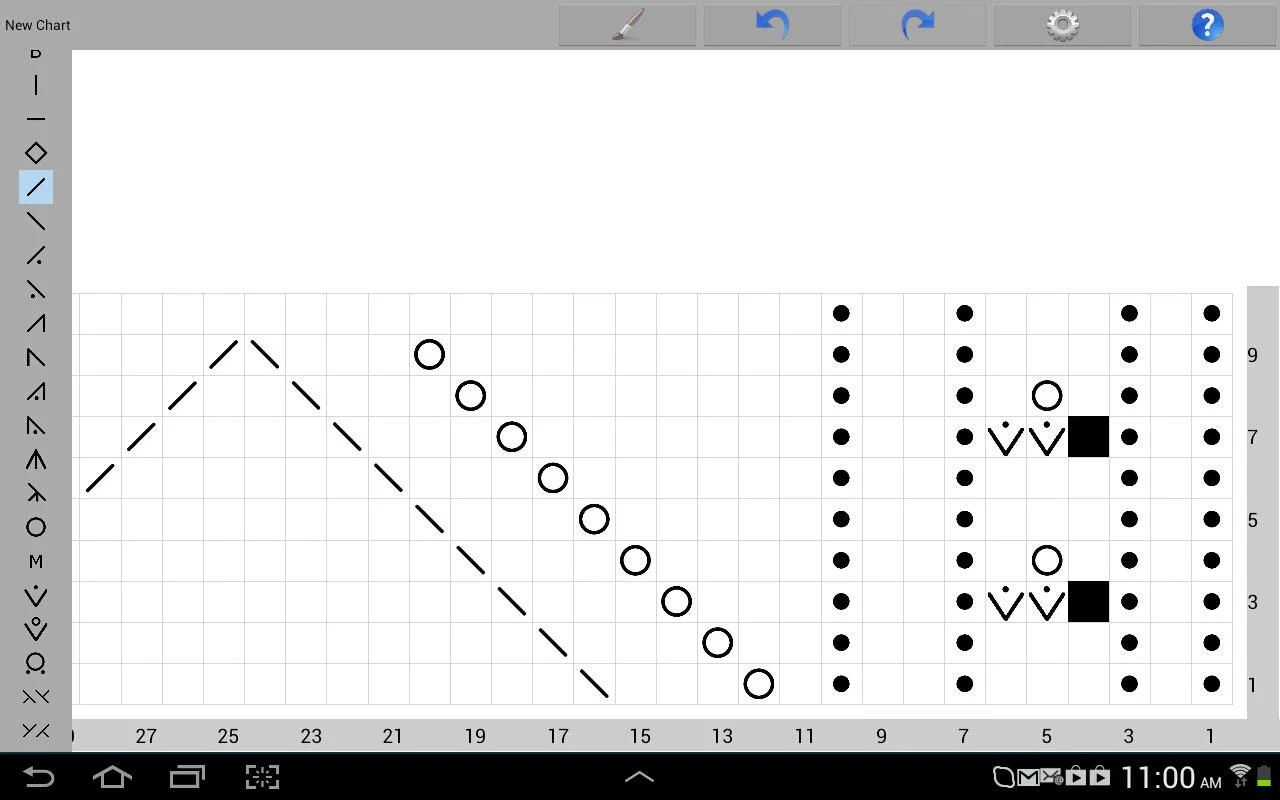
\includegraphics[width=2in]{images/image03.png}
\caption{Chart editor of Knitting Chart Maker}
\label{fig_knittingchartmaker}
\end{center}
\end{figure}

\subsection{Other}

\subsubsection{KnitML by Jonathan Whitall}
KnitML is an XML based format for describing the knitting process from beginning
to the finished product. With KnitML The project aims to establish an
international standard for knitting pattern expression (\url{http://www.knitml.com/blog/static.php?page=about-knitml}).
He aims to do so by using the Knitting Expression Langauge, KEL, that he defined
(\url{http://www.knitml.com/docs/users-guide.html#d0e246}). KEL is based on the
Groovy programming language (\url{http://groovy-lang.org/templating.html}) for
the Java platform and the GroovyMarkup architecture.

The following KEL expression

\begin{lstlisting}
Pattern {
    generalInformation
}
\end{lstlisting}

Would result in

\begin{lstlisting}
<pattern>
    <general-information/>
</pattern>
\end{lstlisting}

The project has not seen updates in any form since 2013 and I presume it
discontinued. A beta of an editor program for KEL and its resulting XML can be
found on the homepage of the project, knitml.com.


\chapter{Requirements}
The requirements for this thesis are formed from user stories from interviews
conducted at the beginning of this thesis. I interviewed three participants
stemming from both my circle of acquaintances as well as from a poster I posted
publicly nearby the HTW’s campuses. Prerequisite for a participant in such an
interview was a proficiency and an interest in knitting. For a transcript of
these interviews consult the appendix A. From these interviews a set of functional
requirements was extracted. \Cref{table_requirements} shows the user stories and
functional requirements extracted.

\newgeometry{margin=2cm}
\begin{landscape}
\begin{table}
\renewcommand{\arraystretch}{1.3}
\caption{Newspapers Studied}
\label{table_requirements}
\centering
\begin{tabular}{ c | p{10cm} | p{10cm} }
\# & User Story & Functional Requirement \\
\hline
1 &
As a knitter I want to be able
to see the knitting pattern chart
 on my phone while knitting &
 Display of knitting pattern chart
that is easily usable while knitting \\
2 & As a knitter I want to create my own charts in the app both in a grid format and a row format & Pattern editor for creating and editing patterns \\
3 & As a knitter I want to transcribe charts from paper into the app with both grid and row formats & Pattern editor \\
4 & As a knitter I want to have a list of all the patterns in the app and add and remove patterns from that list & CRUD for patterns and showing list of patterns \\
5 & As a knitter I want to convert metric units for needle sizes, yarn weight and length to imperial and vice versa Unit converter in app & Unit converter in app  \\
6 & As a knitter I would like to enter a set of written knitting instructions and be able to see each individual instruction while knitting and jump to the next instruction with a button press & Editor for written instructions and view of them to be used while knitting with button or voice command \\
7 & As a knitter I want to use my phone to count the rows I knit & Row counter \\
8 & As a knitter I would like to be able to look up the explanations and visual instructions for different kinds of stitches while inside the app & Glossary of stitches with explanations and instructions \\
9 & As a knitter I want to have a way to jump to the row I'm currently on in my knitting pattern and to get back to the default zoom level & Button for resetting the zoom level and to jump to current row when viewing a pattern \\
10 & As a knitter I want to be able to take pictures of the finished, knitted products of a pattern & In-app camera and function for adding images from disk \\
11 & As a knitter I want to be able to see pictures of the knitted products of a pattern & Gallery for knitted products from a pattern \\
12 & As a knitter I want to have all my knitting projects with their details (pattern, required needle size and yarn, etc.) easily accessible in one app & Knitting project management functions  \\
13 & As a knitter I want to be able to use the row counter with another app in the foreground &  Have row counter increase and decrease button in notification bar when knitting app is not the active app \\
14 & As a knitter I want my screen to stay on until I exit the app & Force screen to stay on while in-app \\
\end{tabular}
\end{table}
\end{landscape}

Within the context of this thesis I focus on the functional requirements \#1, 2, 3, 4, 8, and 7. To summarize, the protoype of the app will present a functioning editor as well as a viewer for pattern charts. Two input styles will be available for both viewer and editor: grid style and row style. The with the editor generated pattern will be stored on disk and will be accessible with CRUD operations within the app. The viewer will have a row counter next to the displayed pattern chart. Buttons for switching between the view styles will be present in the editor as well as the viewer.

After these requirements will have been fulfilled and time allows, further features for the app will be: a button for resetting the zoom level and jumping back to current line in the pattern, a row counter increase and decrease button outside of the app and the option to force the screen to stay awake while within the app.

\chapter{Design}
The desired outcome of this thesis will be an usable Android app with working CRUD functions for knitting chart patterns and row counter functionality while viewing a pattern. This app is intended as an aid for knitters of all backgrounds during their respective knitting projects.

A chart pattern will consist of a set number of rows and columns. Each cell of the grid contains a symbol representing a knitting stitch. Created pattern are stored locally on the device and can be manipulated by the user in-app, as CRUD operations apply. Creating, editing and viewing patterns will be based on two shared visual formats for the pattern: a grid format and a row format.

The grid format will display the pattern in a grid, simulating the most common form of commercial distribution for knitting chart patterns on both analogue and digital media. Manipulation of the pattern content will be possible through a software keyboard containing the stitch symbols. A symbol can be selected and then applied to cells in the grid via touch. The symbol will stay active until the user selects a different symbol. The grid size can be changed with a button which opens a dialog where the desired amount of rows and columns can be entered. On confirmation the grid will shrink or expand to the set dimensions. Any symbols lying outside of the new bounds will be deleted, whereas new cells will be empty.

Similar to the grid format the row format will display the pattern rows, but will forego the representation of the columns. Instead the cells of a row will be summarized in such a way, that consecutive, identical symbols will be represented  by a number value equal to the count of the symbols and followed by the stitch symbol. Rows in this format can be edited like a conventional text editor - a movable cursor to show where further user input will be inserted and text selection functions for multiple character deletion, copying and pasting will be available. The software keyboard corresponding to this format will consist of the stitch symbols and a num pad, as well as an enter and a backspace key.

Viewing a pattern will come with a row counter below the actual chart pattern. This counter can be increased, decreased and reset by utilizing buttons. The current row will be indicated through a highlight on the pattern, marking the corresponding row in both grid and row format.

While editing or viewing a pattern, the row and the grid format will allow the user to 2D scroll, meaning both vertical and horizontal scroll, and zoom the pattern. Switching between both formats while editing and viewing a pattern will be supported with a button. Upon switching the pattern will be saved. Renaming, deleting, and saving the pattern will be possible from within both formats with buttons.

On app launch the list of patterns saved on the device will be shown. A list item will consist of the pattern name, an edit, and a delete button. A click on the pattern name will open the pattern in the viewer in row format with the default dimensions of 10 columns and 10 rows. Below the list will be a button to create a new pattern which will open a dialog for entering the new pattern’s name. After confirming a name, the editor will open with the row format.

\subsection{Wireframes}
\begin{figure}
\centering
\begin{minipage}{.5\textwidth}
  \centering
  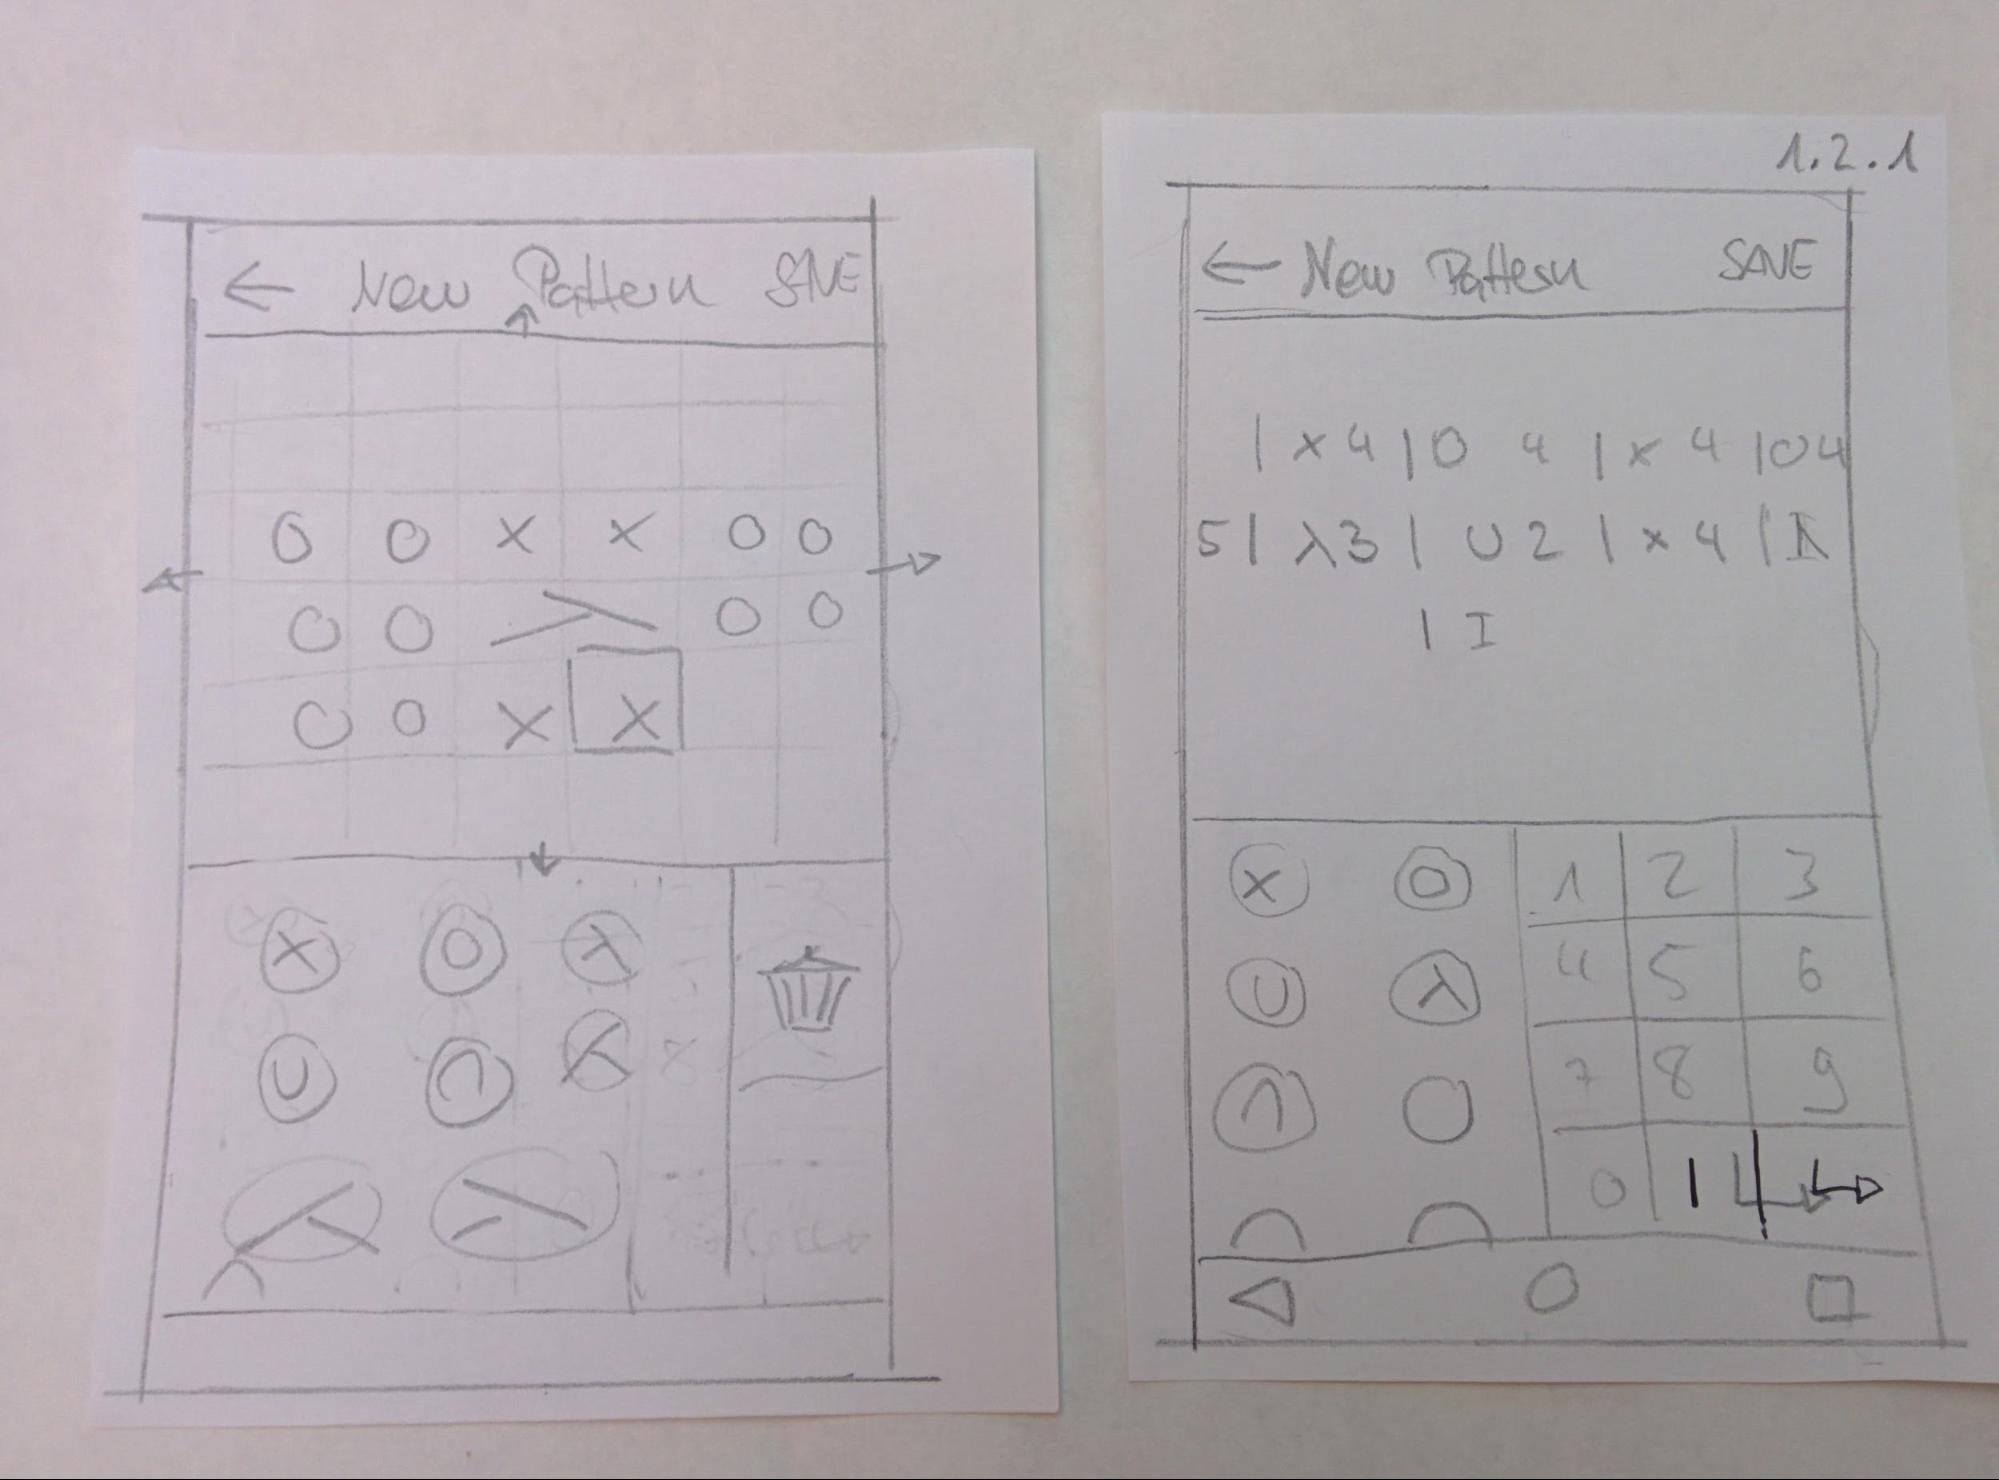
\includegraphics[width=2.5in]{images/image09.jpg}
  \caption{Editor screens for grid and row format with pattern name and save button in navigation bar}
  \label{fig_wireframe1}
\end{minipage}

\begin{minipage}{.5\textwidth}
  \centering
  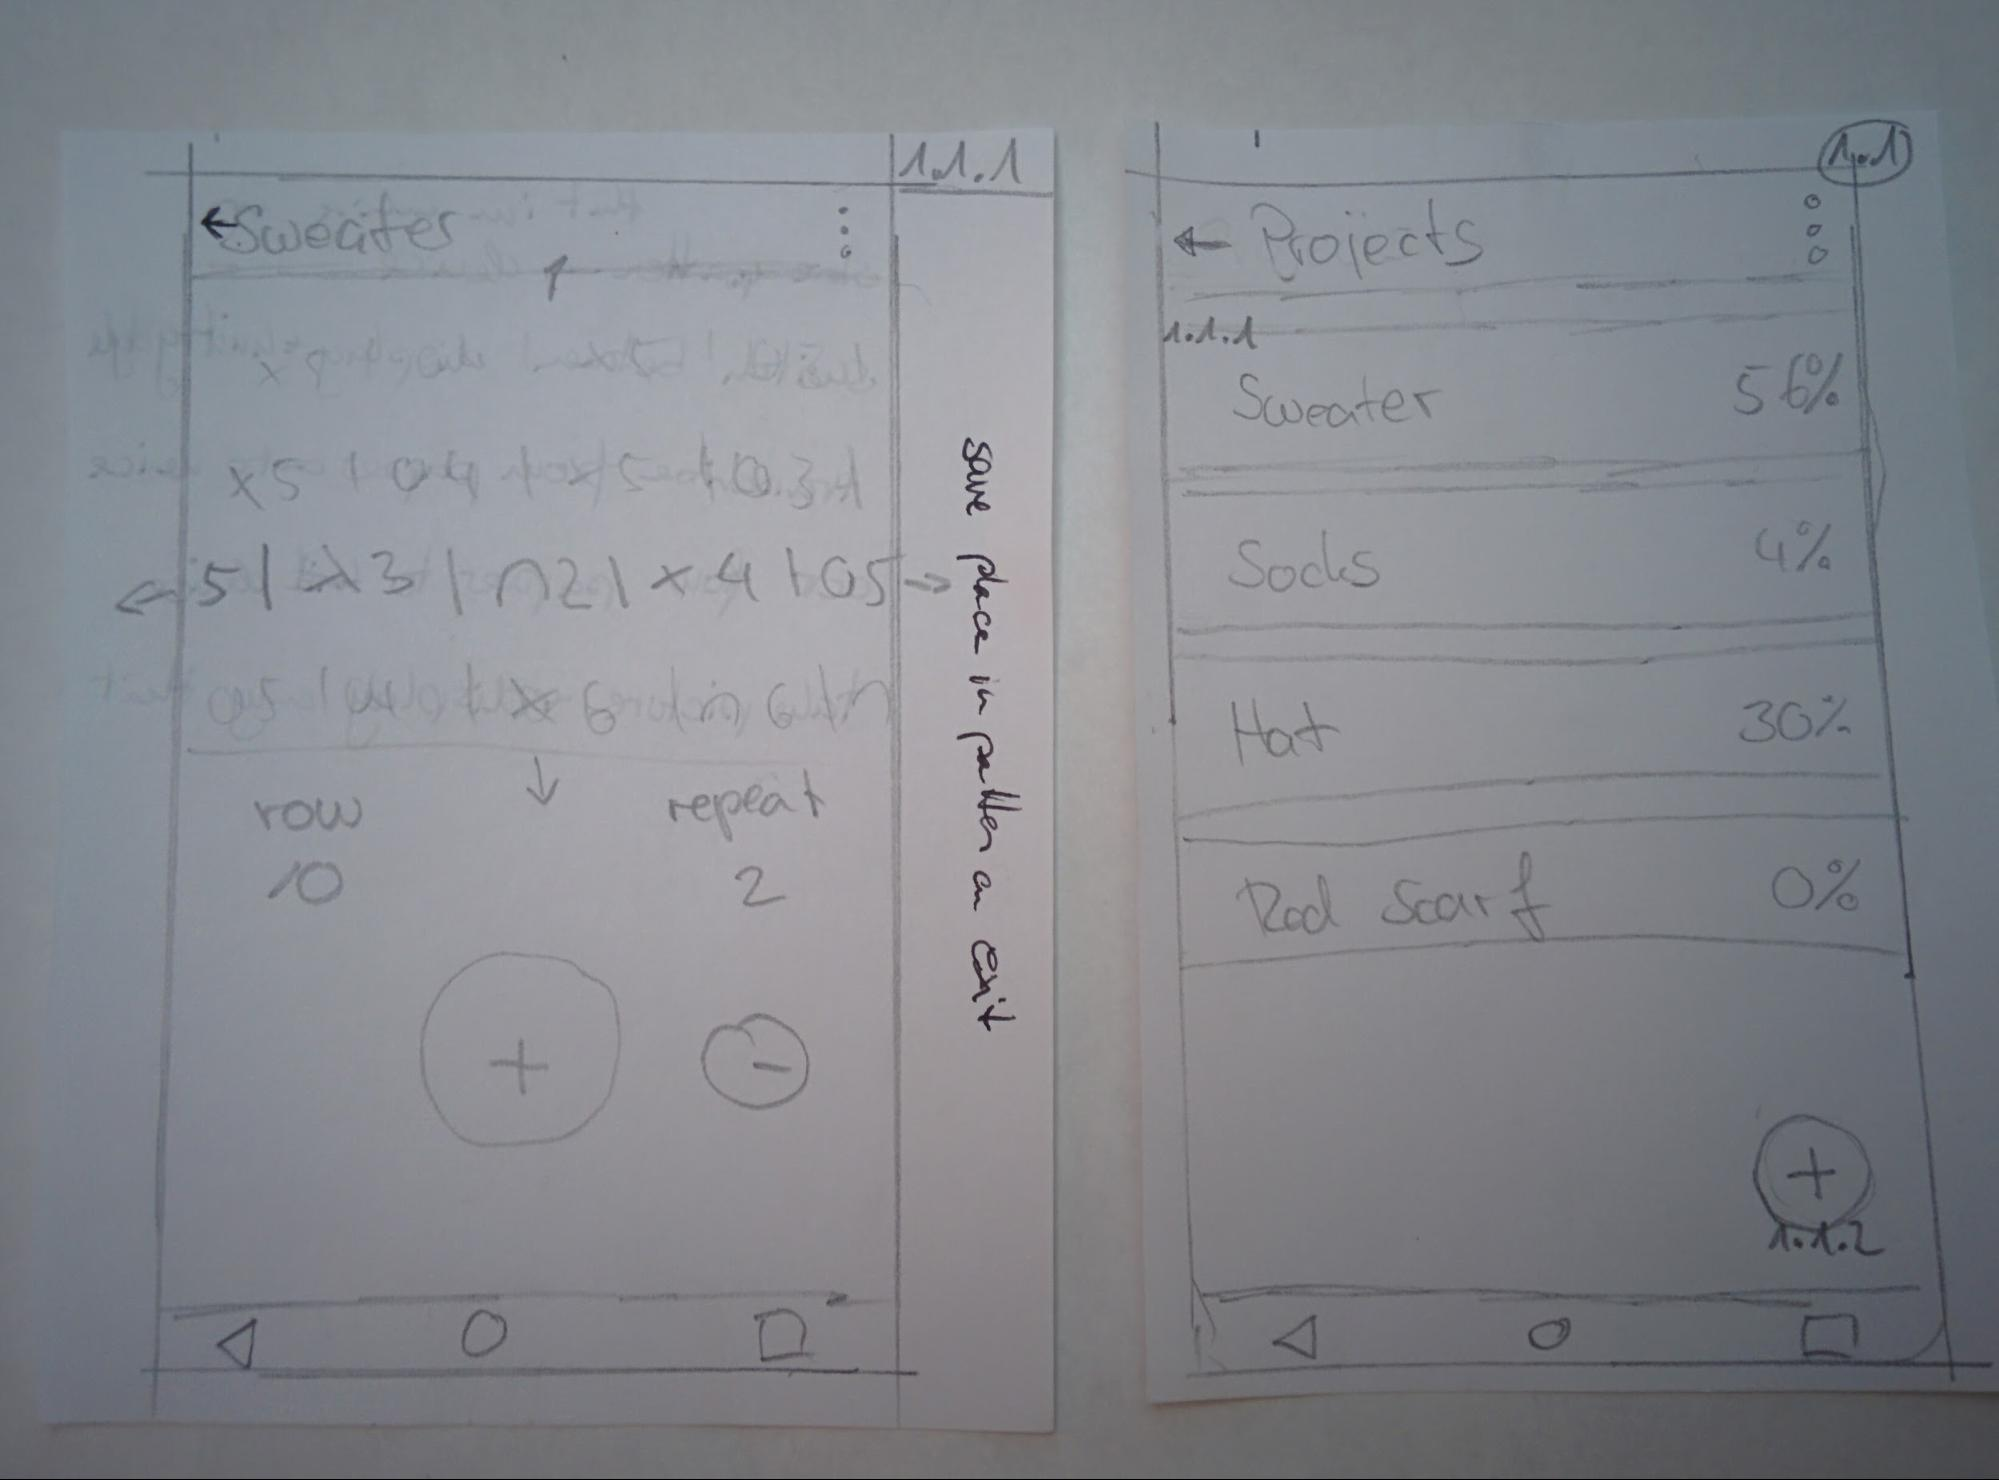
\includegraphics[width=2.5in]{images/image08.jpg}
  \caption{Viewer screen for row format and selection screen for stored patterns}
  \label{fig_wireframe2}
\end{minipage}
\caption{Screens for editor and viewer without Android elements}
\end{figure}

\begin{figure}
\centering
\begin{minipage}{.5\textwidth}
  \centering
  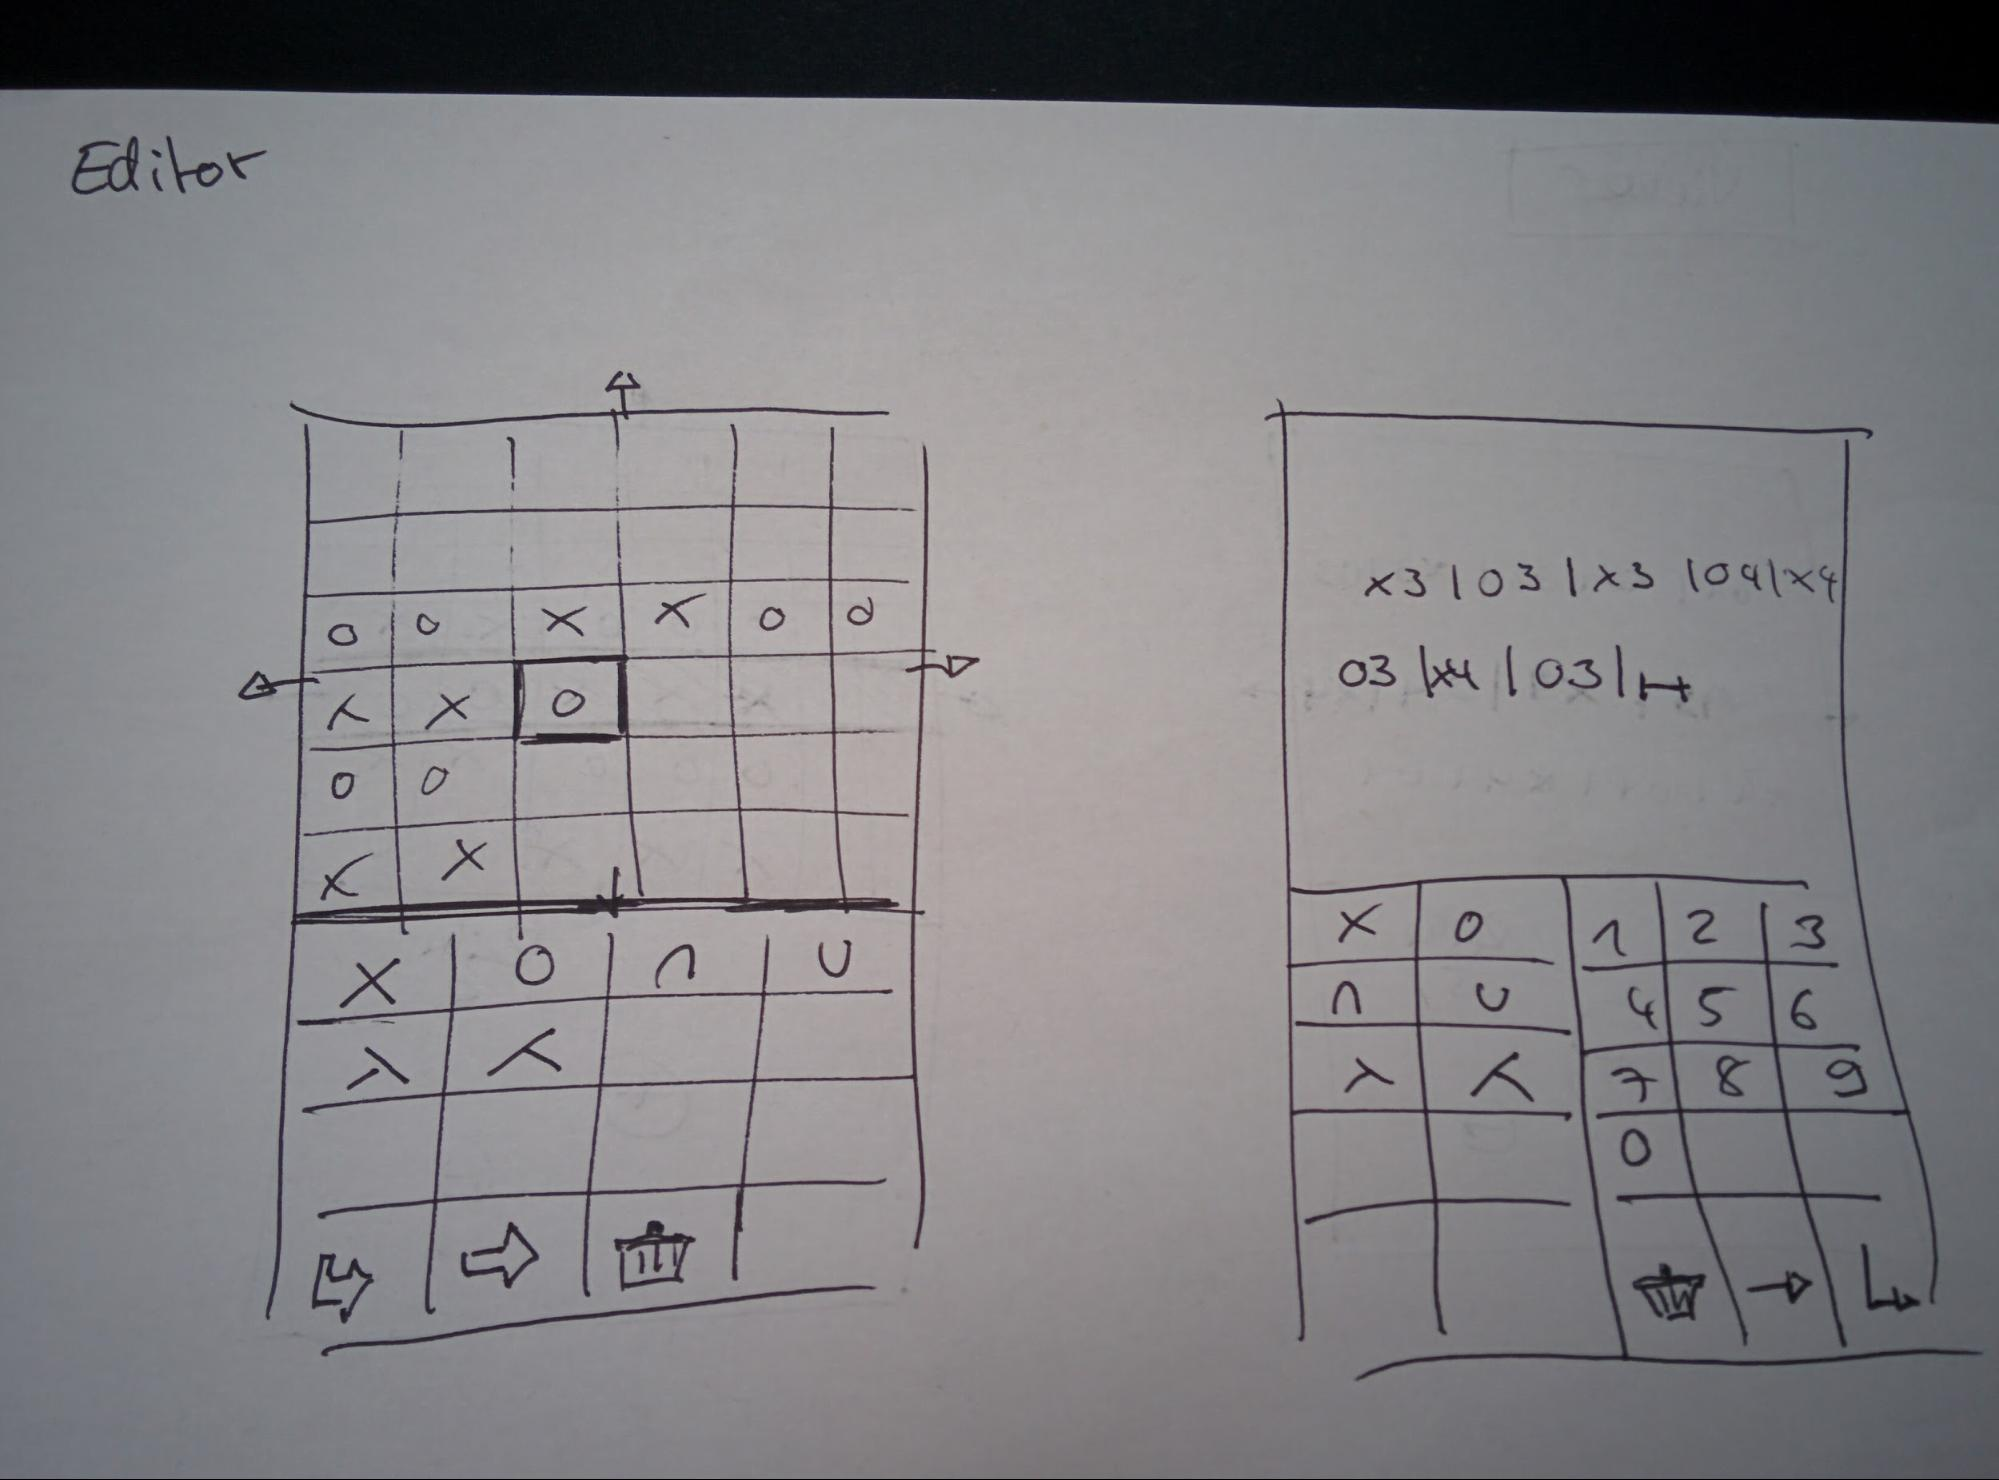
\includegraphics[width=2.5in]{images/image00.jpg}
  \caption{Editor screens for grid and row format}
  \label{fig_wireframe3}
\end{minipage}

\begin{minipage}{.5\textwidth}
  \centering
  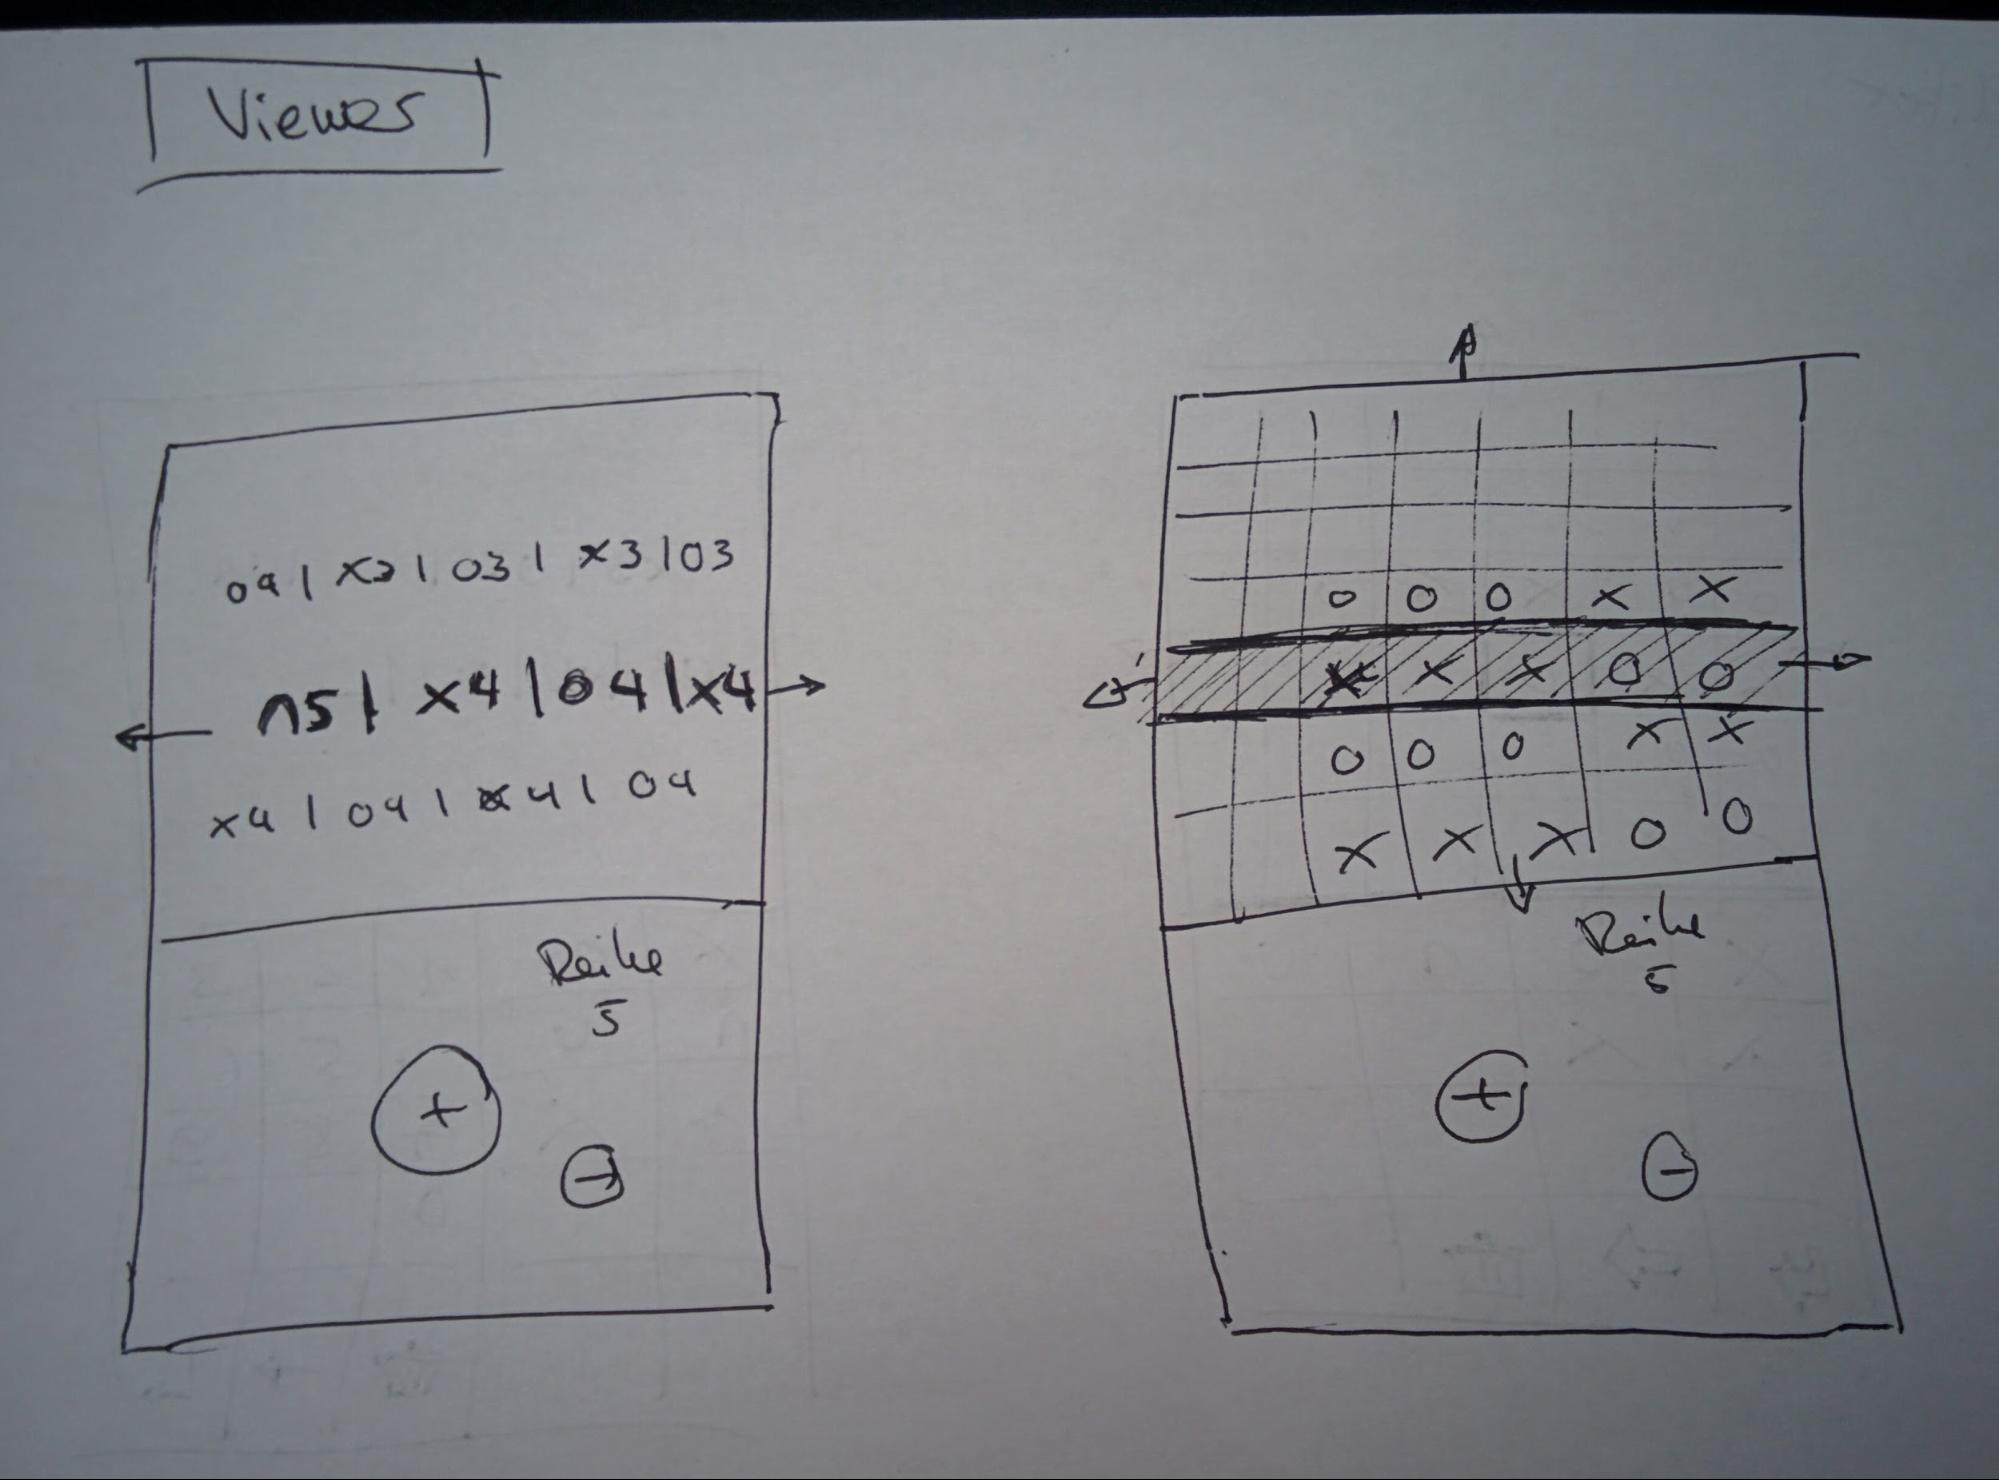
\includegraphics[width=2.5in]{images/image02.jpg}
  \caption{Viewer screens for grid and editor format with row counter}
  \label{fig_wireframe4}
\end{minipage}
\end{figure}

\chapter{Implementation}
\textit{Google’s IDE Android Studio 2.1.2 is used for the implementation of the Android app. }

\section{Basic structure of an Android app}
An Android app consists of at least one activity which can contain one or more fragment --- both are basic Android application components. An activity, in the Android context, is a Java class that extends the Activity class. It manages a screen and is needed to display any user interface. Fragments implement a specific user interface or behaviour and should, ideally, be modular so they can be reused with multiple activities and in different screen configurations. Both components have their own lifecycles and events during the apps runtime. Activities feature methods such as onCreate(), onStart(), onStop(), and onFinish(), which can be overwritten to implement logic that is executed at different points in it’s life. Same applies for a fragment, but where an activity can stand alone, a fragment always needs to be attached to an activity; it is connected to that activity's lifecycle --- is the activity stopped, the fragment will stop as well.
When containing fragments, the activity’s job is that of managing those fragments through getters and setters and orchestrating the communication between fragments, which is done with callbacks defined in the fragments.

Activities and Fragments can house ViewGroups and Views, which define different UI components for Android. Such a view would be a TextView, which displays one multiple lines of text. Viewgroups and views can be extended in custom classes to implement non-standard behaviour.

The implementation part of this thesis will focus on the creation of custom views for Android to display and interact with pattern charts.

\section{Stitch symbols}
There are two possible ways to display a symbol of any kind in views in Android: one is to use drawables, image resources and the other to use text with a custom font. I decided to go with the second approach, since that would allow to save and display patterns using simple strings. Furthermore fonts are rendered during runtime with antialiasing, meaning the quality of the displayed symbol is consistent across screen sizes, whereas with drawables files with different resolutions would be needed to optimize both resources usage when loading the drawables into memory and view quality.
A font consists of glyphs, which contain information how a character is to be displayed. It is also possible to have ligatures in the font, meaning that multiple character in a specific combination will be represented by a single glyph rather than three individual glyphs. Such an example is the String “fi” which displays as “fi” when using the font Roboto. This can be used to display more stitches than there are keys available on the keyboard. To fit the time constraints of this thesis I will limit stitch symbols to single letter glyphs.
I used the open source software Font Forge to create the knitting font for this thesis.

\section{Pattern}
Using a custom font for the stitch symbols allows to represent patterns as combinations of characters. Within the app prototype I use three different pattern formats: one for the Pattern POJO (Plain Old Java Object) which is used for the persistent storage, one for the row format, and one for the grid format.

The grid format uses a two-dimensional String array of columns and rows and can  be likened to the way a pattern chart is displayed on paper. Each cell is filled with a String representing a stitch.

The row format is one String that is used with Android’s EditText widget. The format implements the shortened pattern rows described in the design chapter of this thesis. An EditText can display multiline text and does so by adding a line feed $\\n$ at the appropriate place in the String. Rows can be distinguished by the $\\n$ following a combinations of letters.

The Pattern POJO contains a field for a String Array of pattern chart rows that, like the pure row format, use the shortened rows for representing a pattern.
The pattern is converted between the different formats by using the class KnittingParser. This class provides static methods for the conversion between grid, row and POJO format.

\section{Persistent Disk Storage}
There are multiple ways persistent storage can be implemented in Android. A common choice is to use a SQLite database, which Android natively supports. Another would be to save files to internal or external storage, which many phones have by way of SD card.
I decided to save the patterns as files to internal storage --- the pattern is saved in the default local directory Android gives the app. For this the Pattern POJO is serialized using Google’s JSON library Gson, which handles the writing, reading and conversion of the files to Java objects and vice versa. Gson supports the usage of Java generics and can map JSON data to POJOs while maintaining inheritance hierarchies.

The Pattern POJO defined in the prototype contains fields for the pattern rows, the total number of columns and rows, and the current row from the row counter with getters and setters for all of the fields. A pattern object’s default state after initialization contains a pattern of size 10 x 10 that is filled with  the character representing an empty stitch. The empty stitch character in the prototype is ‘u’.

It inherits from the class Metadata which contains both a UUID representing the pattern id and the name the user gives the pattern. When storing on disk Pattern POJOs are converted to JSON using Gson and saved with the id as filename. The metadata from the pattern is then added to an ArrayList of Metadatas which is saved in the same local app directory and acts as an index of all patterns saved on the device. Using an index file increases performance, since to get a list of the existing patterns not all pattern files have to be loaded, but just the one file containing the ArrayList of Metadatas. Individual pattern can then be loaded using the id saved in the patterns Metadata.

\section{Keyboard}
The row and the grid editor use different keyboards each. The keyboard of the grid editor features stitch symbols and a delete button. The symbols and the delete button can be toggled to be in the active state. While a symbol is active, touching the grid will lead to the active symbol being added to the pattern at the touched cell. Since empty cells contain the designated empty character ‘.’, deletion works in the same way as writing. The keyboard is implemented using a Gridview, a default Android component to display a collection of items in a grid with equal spacing between the items, that also features scrolling. A grid item consists of text set on a KnittingFontButton, a custom view that I defined that extends Android’s own Button view. The custom button sets the custom knitting font defined for the project.

In the row editor there are three sections of the keyboard. One for the symbols, one for numbers and one that includes the enter and backspace buttons. Pressing a symbol and number button will append the character or the number to the editor. The enter and backspace button call the system’s enter and backspace key events from Android’s software keyboard.
The symbols sections is also a Gridview, although with less columns than in the grid editor. For the numpad I use the Viewgroup class CalculatorPadLayout form Rahul Parsani. The viewgroup takes a number of child views, in this case KnittingFontButtons, as well as arguments for row and column count. It then calculates the size of the child views so, that they are all equal in size and distribution. There are multiple reasons for using a custom Viewgroup here instead of a Gridview. A Gridview uses an Adapter class to populate the items in it with a collection and handle the onClick event of these items. It supports changes in the collection and offers methods to notify the adapter to redraw the grid after data changes. Writing such an adapter class is unnecessary since the number buttons in the numpad will not change. Each button also calls the same method, an individual handling of onClick events is therefore superfluous. Additionally, a Gridview always makes its items scrollable by default, something that we don’t want with a numpad even on different screen sizes. A LinearLayout, a Viewgroup that displays its children one after another, either vertically, or horizontally, could be used there too, but would increase the number of layouts that need to be rendered on the screen. That is generally something to avoid, since views are quite resource intensive in Android and can cause lag in the app. Lastly, the enter and backspace buttons are displayed in a single LinearLayout.

All buttons use a drawable for their background to indicate pressed and clicked states with a filled circle round the pressed button.

\section{Grid pattern format: GridEditorView}
For displaying the grid format I first looked into Android’s own grid implementations, the Gridview and the TableLayout. The TableLayout is similar to HTML’s table tag and is displays elements in rows and columns. It should only be used if the underlying views or data will not change. A Gridview, as used for the symbol keyboard, seems an optimal solution for a grid. Unfortunately it is not possible to implement frozen cells, so that the first row and column stick to the edges of the screen to display the row and column numbers.

I then took inspiration from the app Knitting Pattern Maker, introduced in the background section, and Google’s developer guide to dragging and scaling, for which they published a sample project implementing those features on an OpenGL canvas that included axis labels.

For the prototype I implemented my own subclass of View. In it I draw the canvas with the line and row numbers, the lines for the grid and the stitch symbols. For the symbols I use the canvas’ drawText() method, which takes a Paint parameter that has the custom knitting font set. The position of touched cells is calculated from the pixel input of the touch event. The finger pinch zoom is implemented using Android’s ScaleGestureListener interface. The onScale method takes the a ScaleDetector as parameter which contains the coordinates relevant to the scaling and the scale factor. The scale factor from the event is then saved and used when drawing the canvas in onDraw to scale the drawing operations. The SimpleGestureListener interface is used for the two-dimensional dragging of the grid. The dragged distances are clamped in the onScroll method and then applied as translation during the drawing of the canvas.
The GridEditorView also has a method to scroll the current line to the center and draw a highlight on the current row in the onDraw method which are used when the grid is displayed in the viewer.

\section{Row pattern format: RowEditorLinearLayout}
The row editor consists of a the RowLinearLayout class, a custom LinearLayout. This layout implements two-dimensional scrolling which uses a native Scroller. The scroll distance is calculated inside the onTouchEvent method and then scrolled by the scroller. It houses one custom EditTexts, which comes with text operations such as selecting, cut, copy, and pasting and a custom TextView. The layout is set programmatically to extend beyond the visible screen and make itself scrollable when the children are bigger than the visible area.

The LinedEditorEditText extends EditText to draw the background for the odd and even lines and to set the knitting font, as well as the highlight for the current row when in the viewer. On the left of the EditText is the LineNumberTextView, a custom implementation of Android’s TextView that contains the line numbers. When a new line is added to the editor, the line numbers get a line added as well.

\section{Editor Activity}
This activity simply contains a FrameLayout to programmatically add the grid and row editor fragments to is and allow easy switching between the visible fragments. The menu contains buttons for switching the editors, saving, the overflow menu, which are the three vertical dots, and, when the grid is visible, to set the grid size. Buttons for deleting and renaming the pattern are located in the overflow menu.

Before the views are switched the activity calls the savePattern method. This method checks whether the pattern has been edited and then saves it to local storage.
When the user tries exits the activity with the software back button or the home button it is checked again for changes. Are any found then the activity will display a dialog to ask the user if he wants to save the changes before exiting.

\subsection{Editor Fragments}
There are two fragments in the Editor Activity: each of the two editor formats has its own fragment that displays the corresponding keyboard. The fragments handle saving, loading, and updating of the pattern data as well as the keyboard presses.
The grid format fragment also displays the dialog for setting a new grid size.

\section{Viewer Activity}
The Viewer activity houses the row counter a placeholder for the grid and row fragments. The counter consists of a simple TextView and Buttons, which show the current line number and increase or decrease the counter. In the activity’s menu top the user can also scroll to the current line, a feature that only the grid implements so far, and find a button to reset the counter in the overflow menu to the right.

The fragments are set during runtime programmatically and can be switched with a menu button. Both fragments indicate the current row number with a highlight on the row.

\chapter{User Tests}

\chapter{Evaluation}


\chapter{Discussion}

Issues:
Edittext not intended for 2D scrolling
Canvas in grid lags: onDraw naive implementation
Edittext opens softkeyboard: suppressing is awkward and not intended
Grid doesn’t pan
Row editor doesn’t scale
Disk operations do not block UI
Edittext doesn’t read lines correctly
Edittext sets width incorrectly
Orientation change not supported yet
Different screen sizes not supported

Outlook:
Ligatures and multi character stitches
Pattern export
Pictures
Zoom in row editor
Panning in grid editor
Support of bigger dimension with canvas optimization
Focal point when scaling




\bibliography{bib}{}
\bibliographystyle{apalike}
\end{document}
